%%%%%%%%%%%%%%%%%%%%%%%%%%%%%%%%%%%%%%%%%%%%%%%%%%%%%%%%%%%%%%%%%%% 
%                                                                 %
%                            CHAPTER ONE                          %
%                                                                 %
%1.1: Big-picture motivation for design optimization
%1.2: What is PDE-constrained opt and why is it valuable for design?
%1.3: Why are conventional optimization algorithms not well suited for (reduced-space) PDE-constrained opt?
%1.4: Matrix-free NK methods: what are they and what are their advantages over conventional opt
%1.5: What are the challenges with using Matrix-free NK that need to be addressed?
%1.6: Thesis Contributions that relate to the challenges above.
%1.7: Thesis Outline
%%%%%%%%%%%%%%%%%%%%%%%%%%%%%%%%%%%%%%%%%%%%%%%%%%%%%%%%%%%%%%%%%%% 
 
\chapter{INTRODUCTION}\label{chap:1}
 
\section{Motivation}
Global warming has been unequivocally proven by scientific evidence~\cite{nasa_warm}. 
Furthermore, there is also strong evidence that human activities, especially anthropogentic emissions of carbon dioxide (CO2), are the major source of this warming.

Every industry has an ethical responsibility to address climate change, including the air transport industry, which is 
responsible for about $2\%$ of the manmade carbon dioxide (CO2) emissions~\cite{aviation_warm, Penner.1999}. While this percentage may seem small,  
researchers suggest that aviation's share of 
CO2 emissions should be multiplied by 1.9 times~\cite{aviation_warm, Penner.1999} to incorporate the impact of altitude and other emissions, like NOx and water vapors. Furthermore, with the number of passengers increasing at an average of $5\%$ each year~\cite{aviation:co2, aviation_warm}, perhaps more in developing markets, the impact of aviation on the environment will only increase. It is estimated that approximately 27,000 new passenger aircraft will be demanded between now and 2030~\cite{aviation_warm}.  In summary, the total contribution of aviation to human emissions of CO2 and other effects will likely rise to $5\%$ and in a worst-case to $15\%$~\cite{aviation_warm} by 2050. 

In light of these figures, reducing the impact on the environment is becoming a driving factor for future aircraft design~\cite{green_2006}. For example, the Advisory Council for Aeronautics Research in Europe (ACARE) is enforcing strict emission targets in order to reduce CO2 emissions per passenger kilometer by $75\%$, NOx by $90\%$ and perceived noise by $65\%$ by 2050 relative to the year 2000~\cite{SKINNER2018933, euro_commi}. To design future aircraft that meet such targets, the aviation industry needs to consider 
a range of strategies, including improved efficiency through optimization.

\section{PDE-constrained Optimization}
Numerical optimization is a powerful tool that can be used to inform the design of aircraft.  In particular, in aircraft conceptual design stage, engineering design optimization can reveal valuable insights about the design trade-offs and help engineers make detailed and informed decisions. Moreover, optimization is increasingly used during detailed design to refine the shape and structural layout of aircraft.  However, the optimization must be coupled with sufficiently accurate models if the results are to be reliable.  For example, in this work we will consider partial-differential equations (PDEs) models that can capture the complex nonlinear physics present in flight.

Engineering design optimization problems that are governed by PDEs arise in many engineering applications including aerodynamic shape optimization \cite{lambe:2014,lyu2014aerodynamic, Zhang567303}, structural optimization \cite{DBLP:DeckelnickHJ17, lambe:2014, kennedy14}, and thermodynamic optimization \cite{chen1999finite,bejan2000thermodynamic,bejan2012thermodynamic}. 
Figure~\ref{fig:1_mot} shows two examples of PDE-constrained design problems: the first one is an aero-structural optimization problem; the second one is a topology optimization problem. 

\begin{figure}[ht]
\centering
\subfloat[Aero-Structure Optimization~\cite{as_opt}]{
  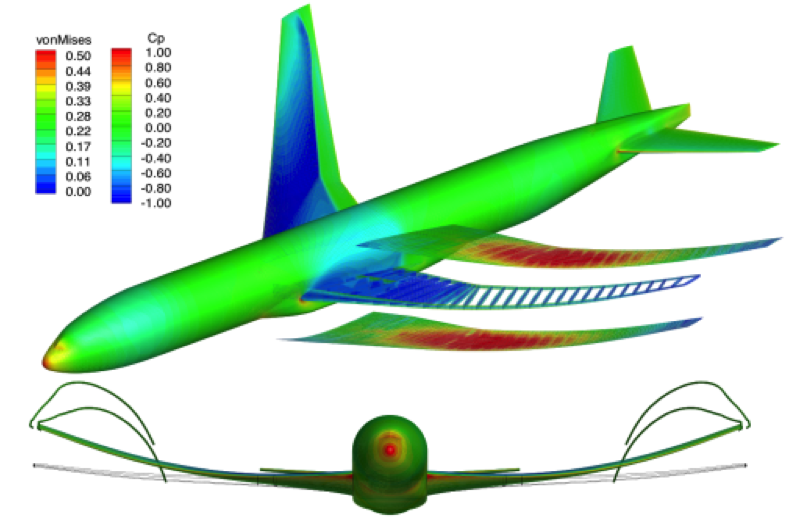
\includegraphics[clip,width=0.6\columnwidth]{./figs/chap1_intro/1_as.png}\label{fig:A}  %
} \\
\subfloat[Topology Optimization~\cite{topo_opt}]{ %
  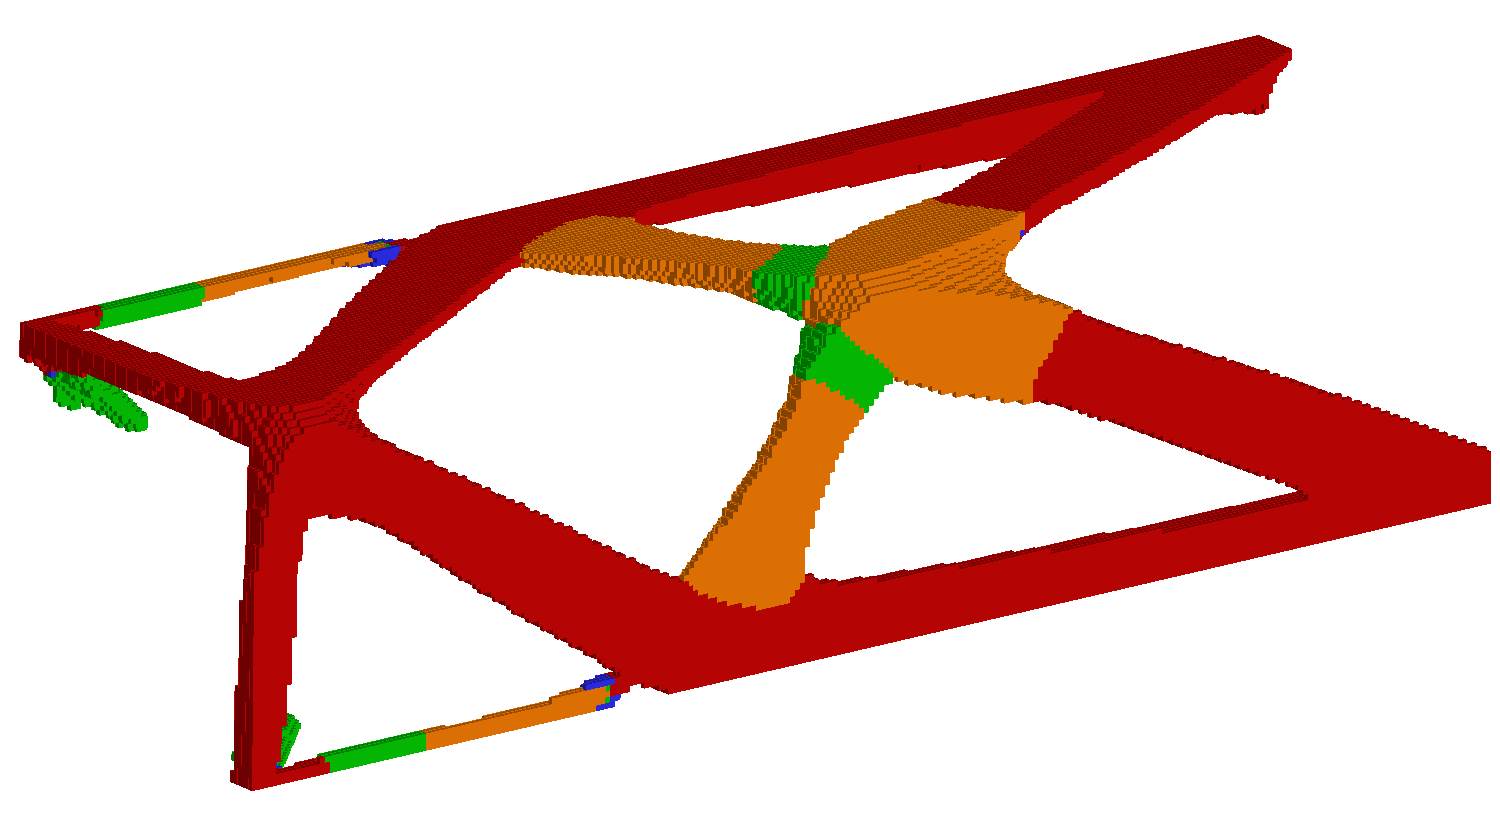
\includegraphics[clip,width=0.6\columnwidth]{./figs/chap1_intro/1_topo.png}\label{fig:B}
}
\caption{Large-Scale PDE-constrained Optimization}
\label{fig:1_mot}
\end{figure}

In PDE-constrained optimization, an optimization library is coupled with one or more PDE models. 
Figure~\ref{fig:outflow} illustrates the schematic diagram of the PDE-constrained optimization process\footnote{More precisely, Figure~\ref{fig:outflow} illustrates a reduced-space PDE-constrained optimization.}.   
As shown in Figure~\ref{fig:outflow}, a typical optimization iteration begins with updating the computational mesh (if necessary), followed by the primal PDE solve. The solution of PDE can then be used to evaluate the objective and constraints.  If a gradient or Jacobian is requested by the optimization algorithm, then one or more adjoint PDEs must be evaluated. 


 \begin{figure}[H]
  \centering
  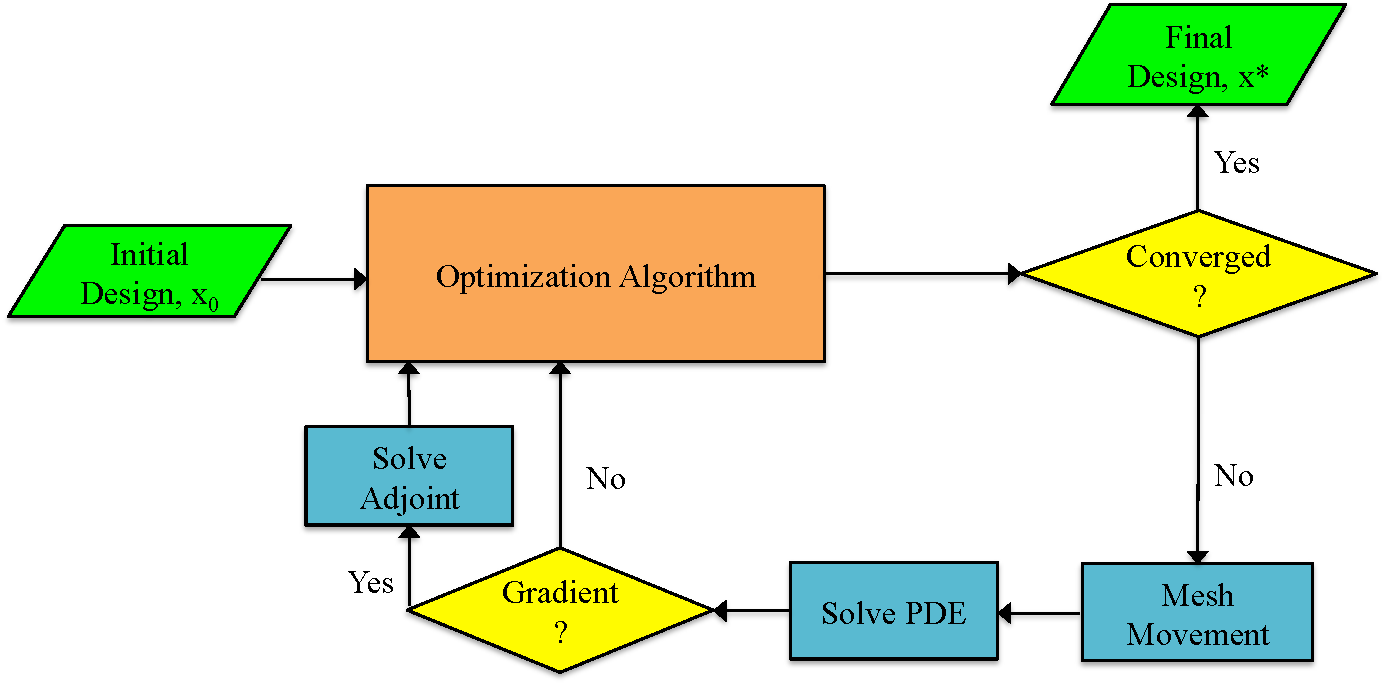
\includegraphics[clip, width=1.0\columnwidth]{./figs/chap1_intro/1_optFlow2.pdf}%  
  \caption{Schematic Process of PDE-constrained Optimization\label{fig:outflow}}
\end{figure}

Computational cost is an important consideration in PDE-constrained optimization.  
Again referring to Figure~\ref{fig:outflow}, we see that each optimization iteration requires the solution of the PDE.  This subproblem itself can be a formidable task in high-performance computing.  Furthermore, gradients and Jacobians require the solution of additional linearized PDEs, \eg adjoints.  In the next section, we will discuss how these differences cause significant challenges for conventional optimization algorithms.

\section{Conventional Optimization Algorithms and Their Limitations}
Conventional gradient-based optimization algorithms~\cite{Nocedal2006NO, Byrd:1999:IPA:588897.589167,gill:2002} have been used extensively in PDE-constrained optimizations, particularly for problems with relatively few  state-based constraints. 
For example, \cite{2015lyu_crm} and \cite{kenway:2014} used SNOPT (Sparse Nonlinear OPTimizer) \cite{gill:2002} through the Python interface pyOpt~\cite{Perez:2011:A} for the investigations of the aerodynamic and aerostructural optimization on the Common Research Model based on RANS. 
Because there were only three state-based outputs of interest, 
drag, lift, and pitch moment coefficients, 
they use adjoint methods~\cite{pironneau:1974, jameson:1988, reuther:1996, Jameson03aerodynamicshape, Mader06adjoint:an,  Lyu2013b, hicken:aiaa2010}  
to assemble the total gradients and feed them to SNOPT.  The cost of an adjoint solution is independent of the number of design variables for each state-based output. 
Other general purpose optimization algorithms, such as IPOPT~\cite{Wachter2006} and Knitro~\cite{Byrd2006}
have been used for aerodynamic design problems~\cite{Lyu2014f, Rumpfkeil2009OptimizationbasedMA} as well. 

However, conventional optimization algorithms are not well suited for large-scale PDE-constrained optimization problems with many design variables and  
state-based constraints. Large-scale problems with many (thousands or more) design variables are a problem, because conventional optimization algorithms typically rely on limited-memory quasi-Newton methods, which have linear asymptotic convergence rates~\cite{liu:1989}. Furthermore, in the presence of many state-based constraints, assembling the total constraint Jacobians can become prohibitively expensive, as each constraint gradient requires the solution of an adjoint equation whose cost is 
comparable to that of the governing PDE. 

This work is particularly concerned with addressing the costs associated with the constraint Jacobian.
Conventional optimization methods require the explicit constraint Jacobian at every major iteration in order to 
factor the matrix and determine a basis for its null-space; this basis is required by many algorithms for constrained optimization~\cite{nocedal:2006}. As already explained, these matrix-based algorithms are not practical when many constraints are present.  Therefore, a different class of algorithm is needed.

\section{PDE-constrained Optimization Algorithms}
\subsection{Full-space and Reduced-space Approaches}\label{sec:pde_mot}
There are two broad classes of algorithm used to solve PDE-constrained optimization problems: full-space methods and reduced-space methods. In order to describe these two approaches and their relative merits, 
consider the following generic PDE-constrained optimization problem, 
\begin{equation}\label{eq:gen1}
\begin{aligned}
\underset{x,u}{\text{min}} \quad &f(x, u) &\\
\text{subject to} \quad &  h(x,u) &= 0  \\
 &  g(x,u) &\geq 0  \\
\text{governed by} \quad &  \mathcal{R}(x, u) &= 0, \\
\end{aligned}
\end{equation}
where $x \in \mathbb{R}^n \ \text{and}\ u \in \mathbb{R}^v$ are the design and state vectors, respectively, and $f: 
\mathbb{R}^n \times \mathbb{R}^v \rightarrow \mathbb{R},  h: \mathbb{R}^n \times \mathbb{R}^v \rightarrow \mathbb{R}^l,  g: \mathbb{R}^n \times \mathbb{R}^v \rightarrow \mathbb{R}^m$ are the objective, equality and inequality constraints, respectively. We assume that $f$, $h$ and $g$ have continuous second derivatives. Finally, $\mathcal{R}(x, u)$ represents the PDE modeling the physical system.

A solution to~\eqref{eq:gen1} must satisfy the first-order necessary optimaltiy conditions~\cite{Nocedal2006NO}.  These conditions are most easily expressed in terms of the Lagrangian, which is the scalar function defined below:
\begin{equation}\label{eq:lag}
\mathcal{L}(x, u, \psi, s, \lambda_h, \lambda_g) = f(x,u) + \lambda_h^T h(x, u) + \lambda_g^T (g(x,u)-s) + \psi^T \mathcal{R}(x,u),
\end{equation} 
where $s \in \mathbb{R}^m$ are the so-called slack variables,  and $\lambda_h \in  \mathbb{R}^l$ and  $\lambda_g \in  \mathbb{R}^m$ are the Lagrangian multipliers for the equality and inequality constraints, respectively. 

Using $\mathcal{L}$, the first-order necessary conditions, as known as 
 the \textit{Karush-Kuhn-Tucker} (KKT) optimality conditions, for \eqref{eq:gen1} can be expressed as
\begin{equation}\label{eq:kktcond}
\begin{aligned}
\partial_x \mathcal{L} &= \partial_x f + \lambda_h^T \partial_x h + \lambda_g^T \partial_x g + \psi^T \partial_x\mathcal{R} = 0, \\
\partial_u \mathcal{L} &= \partial_u f + \lambda_h^T \partial_u h + \lambda_g^T \partial_u g + \psi^T \partial_u\mathcal{R} = 0, \\
\partial_{\psi} \mathcal{L} &= \mathcal{R} = 0, \\
\partial_{\lambda_h} \mathcal{L} &= h = 0, \\
\partial_{\lambda_g} \mathcal{L} &= g - s = 0, \\
-\mathsf{S} \mathsf{\Lambda}_g e &= 0,\\
s \geq 0, &\quad \lambda_g \leq 0. \\
\end{aligned}
\end{equation}
For notational convenience, we have  introduced $e = [1,1,\ldots,1]^T$ and the diagonal
matrices
\begin{equation*}
  \mathsf{S} = \mydiag\left(s_1,s_2,\ldots,s_m\right),\qquad\text{and}\qquad
  \mathsf{\Lambda}_g = \mydiag\left(\lambda_{g1}, \lambda_{g2}, \ldots, \lambda_{gm}\right).
\end{equation*}

As mentioned earlier, the nonlinear system \eqref{eq:kktcond} can be solved in either the full space or the reduced space.  Full-space methods~\cite{DBLP:journals/siamsc/BirosG05,DBLP:journals/siamsc/BirosG05a,haber:2001} solve all the unknowns in \eqref{eq:kktcond} simultaneously. This results in a large nonlinear system whose size is more than double the number of PDE state variables (due to the adjoint).  If Newton's method is used to solve~\eqref{eq:kktcond}, the resulting linear system is highly sparse, indefinite, and ill-conditioned. Nevertheless, effective iterative methods and preconditioners have been proposed for full-space methods~\cite{DBLP:journals/siamsc/BirosG05, DBLP:journals/siamsc/BirosG05a}.

An advantage of the full-space approach is that, 
during the intermediate optimization iterations, the PDE state equation, $\mathcal{R} =0$, and adjoint equation, $\partial_u \mathcal{L} = 0$, do not need to be solved exactly. This avoids the computational expense of tightly converging the PDE and adjoint equation residuals; however, this is also a potential disadvantage in practical engineering problems, because, if the optimization fails to converge, the intermediate solution may not be feasible with respect to the physics.  Furthermore, for highly nonlinear PDEs, \eg gas dynamics with shocks and boundary layers, practitioners have developed specialized globalization strategies that may be difficult to take advantage of in general-purpose full-space optimization algorithms.  For theses reasons, no general purpose optimization libraries exist for full-space methods, to the best of our knowledge.

%Newton-based full-space methods possess good scaling, but are complicated to implement as they require intrusion to the PDE solver. 
Reduced-Space algorithms for solving~\eqref{eq:kktcond}  
treat the states $u$ and the adjoints $\psi$ as implicit functions of the design variables through $\mathcal{R}(x,u(x)) = 0$, and $\partial_u \mathcal{L} = 0$. Consequently, the reduced KKT conditions can be formulated as follows:
\begin{equation}\label{eq:opt00x}
 \begin{gathered}
    F(x,s,\lambda_h, \lambda_g) \equiv 
    \begin{bmatrix}
\nabla_x f + \lambda_h^T \nabla_x h + \lambda_g^T \nabla_x g\\
-\mathsf{S} \mathsf{\Lambda}_g e\\
h  \\
g - s 
\end{bmatrix} =0,\\
\text{subject to} \quad s_i \geq 0, \quad \text{and} \quad \lambda_{gi} \leq 0 \qquad \forall i = 1,2,\ldots,m, \\
\end{gathered}
\end{equation}
where the unknowns are $x^T, s^T, \lambda_h^T, \lambda_g^T$, 
and $F :\mathbb{R}^{N} \rightarrow \mathbb{R}^{N}, N=n+l+2m, $  
 is the vector-valued residual
of the KKT conditions, excluding the inequalities on $s$ and $\lambda_g$.  

The reduced-space approach to PDE-constrained optimization is attractive for a few reasons.  First, it should be clear that the KKT system~\eqref{eq:opt00x} is much smaller than~\eqref{eq:kktcond}.  Second, reduced-space algorithms are more modular, since they can make direct use of existing PDE primal and adjont solvers.  
This modularity is one of the reasons that the reduced-space approach has remained the dominant approach in aerospace applications. 

Of course, the reduced-space approach is not without difficulties.  If conventional optimization algorithms are used to solve~\eqref{eq:opt00x}, then the aforementioned scaling issues arise, particularly the cost of evaluating the explicit constraint Jacobian.  Instead, we need an algorithm that does not require the explicit constraint Jacobian.
%%%%%%%%%
%The challenges include globalization, which refers to the ability to bypass local minimizers, and nonconvexity handling, which involves bypassing maximizers. The first challenge is addressed in Chapter~\ref{chap:homotopy} and the second in Chapter~\ref{chap:linsys}. 

\subsection{Reduced-Space Inexact-Newton Methods}
One alternative to using conventional (matrix-based) optimization algorithms 
to solve the reduced-space KKT conditions \eqref{eq:opt00x} 
is to apply inexact-Newton methods~\cite{dembo:1982},
which are also know as truncated-Newton methods in the optimization
literature~\cite{nash:2000}.  

To see how inexact-Newton methods can be used to solve~\ref{eq:opt00x}, notice that, 
with the exception of the bounds on $s$ and $\lambda_g$, the KKT conditions
\eqref{eq:opt00x} form a set of nonlinear algebraic equations, $F(q)=0$, 
where $q \equiv (x^T, s^T,
\lambda_h^T, \lambda_g^T)^T \in \mathbb{R}^{N}$ is the vector of unknowns.
These equations can be solved, in principle, using Newton iterations of the form
\begin{equation}
(\nabla_q F) \Delta q^{(k)} = -F(q^{(k)}), \label{eq:Newton}
\end{equation}
where $q^{(k)}$ is the solution at the $k$th iteration and $\Delta q^{(k)} =
q^{(k+1)} - q ^{(k)}$ is the solution update.  Solving~\eqref{eq:Newton} exactly
can be inefficient during early Newton iterates when the linear model is not a
good approximation to $F(q)=0$.  Instead, truncated- and inexact-Newton methods
find approximate solutions to \eqref{eq:Newton} that, for example, satisfy the
inexact-Newton condition
\begin{equation}
  \left\| (\nabla_q F) \Delta q^{(k)} + F(q^{(k)}) \right\| \leq \eta_k \left\| F(q^{(k)}) \right\|, \label{eq:inexact_Newton}
\end{equation}
for some parameter $\eta_k \in (0,1)$.


There has been considerable success applying inexact-Newton methods to
unconstrained optimization problems; see \cite{nash:2000} and the references
therein.  On the other hand, inexact-Newton methods for general (nonconvex)
constrained problems are much less common.  Some notable exceptions include the
efforts by Byrd and colleagues~\cite{byrd:2008, byrd:2010} and by Heinkenschloss
and Ridzal~\cite{heinkenschloss:2014}; however, these algorithms make
assumptions regarding the structure of the problem that favor full-space
formulations, and our experience applying them to reduced-space PDE-constrainted
optimization has been disappointing.

Applying Newton's method to \eqref{eq:opt00x}, the KKT system, also called the primal-dual system, is obtained:
\begin{equation}\label{eq:kkt0}
\begin{bmatrix} \nabla_{xx} \mathcal{L} & 0 & \nabla_x h^T  & \nabla_x g^T  \\
    0 & -\mathsf{\Lambda}_g & 0 & -\mathsf{S} \\
     \nabla_x h & 0 & 0 & 0 \\
    \nabla_x g & -\mathsf{I} & 0 & 0 
    \end{bmatrix}
    \begin{bmatrix} p_x \\ p_s \\ p_h \\ p_g \end{bmatrix}
    = - \begin{bmatrix} \nabla_x \mathcal{L} \\ -\mathsf{S} \mathsf{\Lambda}_g e \\ h \\ g - s \end{bmatrix}
\end{equation}
where $\mathcal{L}$ the Lagrangian is defined in \eqref{eq:lag}, and $\mathsf{S}$ and $\mathsf{\Lambda}_g$ are as defined previously. 
A Newton-Krylov (NK) algorithm is a type of inexact-Newton method that solves~\eqref{eq:kkt0} 
approximately using a Krylov iterative method, which only needs the matrix-vector product of the system matrix. The products can be formed in a matrix-free way by solving two second-adjoint systems; for details, see~\cite{hicken:inexact2014, dener:idf2017} and the references therein.  
This is significant, because it means that NK algorithms do not require the constraint Jacobian (or Lagrangian Hessian) explicitly, unlike conventional optimization algorithms.

%%However, while NK methods can avoid the cost associated with forming the explicit constraint Jacobian, the extension to inequality constraints faces several significant challenges. First, active-set and interior-point algorithms that make use of an explicit basis for the null space of the constraint Jacobian cannot be used, because such a basis requires the Jacobian to be explicitly available.  Second, the primal-dual saddle-point system raised in optimization is indefinite and ill-conditioned, making it difficult for iterative Krylov methods to converge to a sufficient tolerance, hurting the convergence rate of Newton's method. Third, dealing with nonconvex Hessian of the Lagrangian in the null space of the constraint Jacobian is also a non-trivial task. 


Prior to this work, the reduced-space Newton-Krylov method has 
been successfully applied to unconstrained problems and certain types of equality-constrained problems. 
In the case of unconstrained problems, a Newton-Conjugate-Gradient method can be used, in which the Steinhaug-Toint variant of CG is used to deal with nonconvex objectives; 
see, for example, \cite{akcelik:2006, Heinkenschloss:1999:IOA, hinze2010optimization,borzi:2011}. 
Reduced-space NK optimization algorithms have also shown promise for some types of equality-constrained 
problems, because,  as already mentioned above, 
they do not require the constraint Jacobian to be form explicitly and, thus, avoid the scaling issue described earlier.  For instance, \cite{dener:idf2017} applied a matrix-free NK algorithm to a class of equality-constrained optimization problems that arise in multidisciplinary design optimization and would otherwise be intractable with conventional matrix-based algorithms.


\subsection{Challenges in Using Reduced-Space Newton-Krylov Methods}
Motivated by its success in the unconstrained and equality-constrained cases, this thesis aims to extend the Newton Krylov methodology to more general, equality and inequality constrained problems. 
This extension of the reduced-space NK algorithm encounters two fundamental challenges that must be addressed.

\begin{description}
\item[Nonconvexity:] The system $F(q) =0$ does not distinguish between different
  types of stationary points, so Newton-type methods, including inexact-Newton-Krylov methods, 
  may converge to local
  maximizers or saddle points.  Conventional optimization algorithms often
  project onto the null-space of the (active) constraint Jacobian to detect
  directions of negative curvature and avoid undesirable stationary points; however, 
  the null-space is not explicitly available for matrix-free inexact-Newton
  methods. Consequently, we must find a matrix-free approach to deal with nonconvexity.
\item[Preconditioning:] The number of iterations necessary to satisfy the
  inexact Newton condition \eqref{eq:inexact_Newton} using a
  Krylov method is closely related to the condition number of the system.
  Unfortunately, it is well known that the primal-dual matrix $\nabla_q
  F$ is indefinite and highly ill-conditioned.  A preconditioner is needed that
  is inexpensive to form, store, and apply.  A general-purpose, inexpensive
  preconditioner is especially difficult to find in the reduced-space context,
  since approximations to $\nabla_q F$ are not readily available as they are in
  the full-space.
\end{description}


\section{Contributions}
This thesis proposes a matrix-free inexact-Newton-Krylov 
optimization algorithm that is specifically intended for large-scale, reduced-space 
 PDE-constrained design problems. 
 The primary contributions of this work are in addressing the challenges 
 related to nonconvexity and matrix-free preconditioning. 

The approach to addressing nonconvexity is to introduce a homotopy map that
implicitly defines a solution curve that connects the solution to an easy
problem to the solution of the desired problem.  A 
predictor-corrector algorithm is proposed to follow the curve from the easy to the desired
solution.  

To address the conditioning of the KKT matrix, a low-rank approximation of 
the Schur complement of the KKT system is proposed. The low-rank approximation 
is computed by using the Lanczos method, which only involves matrix-vector products with the Schur 
complement. The matrix-vector products can be obtained using approximate state and adjoint solutions. 

\section{Thesis Outline}
The remaining chapters in the thesis are structured as follows: 
\begin{itemize}

\item Chapter~\ref{chap:homotopy} reviews the homotopy-based globalization and the homotopy map adopted in this work. Then it describes the predictor-corrector path-following algorithm that traces the homotopy zero curve. Finally, the proposed algorithm is verified and investigated using analytical problems.

\item Chapter~\ref{chap:linsys} is focused on describing the proposed matrix-free preconditioner.
It begins by considering inequality constrained problems, and then generalizes the preconditioner to 
problems with both equality and inequality constraints. A synthetic quadratic problem with linear inequality constraints is used to investigate the effectiveness of the inequality preconditioner and the scalability performance of the algorithm. 

\item Chapter~\ref{chap:tests} presents the main numerical results.  The chapter begins by describing the
optimization environment Kona in which the proposed algorithms have been implemented.  Subsequently, the chapter summarizes a state-of-the-art optimization algorithm (SNOPT) against which comparisons will be made.  The predictor-corrector algorithm and the preconditioners 
are first tested on a subset of the CUTEr problems. Next, the proposed algorithms are applied to the stress-constrained mass minimization of a flat plate. Finally, we present the results of a three-dimensional aerodynamic shape optimization problem. 
 
\item Chapter~\ref{chap:con} provides conclusions and some recommendations. 
\end{itemize}


%For PDE-constrained optimization problems, when there are many state-based constraints, assembling the total constraint Jacobian is very expensive as it demands an adjoint solve for each state-based constraint. Additionally, general optimization algorithms store the constraint Jacobians at each design point, which puts a heavy memory load on the computer. Therefore, most general optimization algorithms possess poor scaling qualities.  
%The first aerodynamic optimization was done in \cite{hicks:1974} by using finite-difference approximations to calculate the gradients. The cost of computing the gradients using finite-difference methods increases drastically as the design dimension increases. The adjoint methods have greatly propelled the advancement of research in aerodynamic shape optimization field. Adjoint methods address the dimensionality issue of finite-differences with a cost independent of the number of design variables. \cite{pironneau:1974} developed the adjoint method for Stokes equations and the incompressible Euler equations, and used the adjoints to optimize airfoil profiles. \cite{reuther:1996} used an adjoint algorithm based on Euler to optimize a complete aircraft configurations.  \cite{jameson:1988} derived the adjoint equations for inviscid compressible Navier-Stokes equations, making it possible to do transonic aerodynamic optimizations.  The discrete adjoint method is more preferred in aerospace optimization as the sensitivities are exact to the discretized objective function~\cite{frank:1992}. \cite{Mader06adjoint:an} derived a discrete adjoint method for Euler equations using automatic differentiation. \cite{Lyu2013b} extended the previous adjoint implementation to 
%Reynolds-averaged Navier-Stokes (RANS) equations and effectively applied it to high-fidelity optimization. \cite{hicken:aiaa2010} developed similar methods for non-planar wings high-fidelity aerodynamic optimization. 



%The simulation problem solves the PDEs for state variables, e.g. the pressure distribution along the surface mesh node points on the wing in Figure~\ref{fig:A}, and the displacement distribution among the solid mesh node points in Figure~\ref{fig:B}, at certain design variables. 

%The performance of the physics system is evaluated in the form of objective function bounded by certain constraints, while the objective and the constraints depend on both the state variables and the design variables. The optimizer will choose a design point, inquire the PDE solver for state variables, and compute the functional values and the gradients of the objective and constraints at that point. 

%The optimizer will process all the information and yield a better design point using mathematical algorithms. The process is repeated until certain criteria is met for optimality.  



% \section{Optimization Algorithms}

%Conventionally, solving general constrained optimization problems without PDE constraints involves forming the Lagrangian, and finding the minimization point of the Lagrangian, which is equivalent to solving the first-order optimality conditions or the KKT conditions. Prevalent sequential quadratic programming methods or newton-type methods for solving a system of equations would further break it down to solving a series of systems of linearized equations, also called the Karush-Kuhn-Tucker (KKT) system. The KKT matrix contains the Hessian of the Lagrangian, which is often approximated using quasi-Newton method, and the total constraint Jacobians, which is straightforward to compute using automatic differentiation or complex step methods. Conventional matrix-based optimization algorithms would use direct factorization methods to solve the KKT system.    

%The kernel of reduced-space Newton-Krylov methods for PDE-constrained optimization solves a series of linear systems, which are saddle point systems, but much smaller than the saddle-point system raised in full-space methods.  Because the solution to the optimization problem \eqref{eq:opt00x} is a saddle point for the Lagrangian \eqref{eq:lag} in that the optimal design point minimizes the Lagrangian, while the optimal multipliers maximizes the Lagrangian ~\cite{benzi2005numerical}.  


%%%%%%%%%%%%

% a popular large-scale matrix-based active -set augmented-Lagrangian optimization method SNOPT.  

%\begin{equation}\label{eq:saddle}
%\mathsf{A} = \begin{bmatrix}
%A & B \\
%C & D
%\end{bmatrix}
%\end{equation}
%One type of Schur complement can be obtained by performing the following LDU decomposition 
%\begin{equation}\label{eq:saddle:ldu}
%\mathsf{A} = \begin{bmatrix}
%A & B \\
%C & D
%\end{bmatrix} = 
%\begin{bmatrix}
%I_p & BD^{-1} \\
%0 & I_q
%\end{bmatrix}
%\begin{bmatrix}
%A-BD^{-1}C  & 0 \\
%0  & D 
%\end{bmatrix}
%\begin{bmatrix}
%I_p  & 0 \\
%D^{-1}C  & I_q 
%\end{bmatrix}
%\end{equation}

% which is indefinite, poor spectral properties (ill-conditioned) 
% Direct solvers, however, are still the preferred method in optimization and other areas. Furthermore, direct methods are often used in the solution of subproblems, for example as part of a preconditioner solve.
%The preconditioners developed here are tailored for PDE-constrained optimization problem. 
% matrix-vector products with A can be performed efficiently
% approximate its action on a vector with (nearly) linear complexity,
% the convergence of the iterates to the optimal solution of problem
% gain efficient, save on storage
%words from the paper ~\cite{benzi2005numerical} Benzi block preconditioners, 
% As the iterates approaches the solution,  the entries in A tend to zero, or infinity, KKT matrix ill-conditioned
% the norm of the inverse Schur complement goes to infinity

% Schur complement reduction 
% null space methods, the null space of the constraint Jacobian, the column of Z span the null space of constraint Jacobian
% popular in optimization, projection of the problem onto the constraint set; 

 
%%% Local Variables: 
%%% mode: latex
%%% TeX-master: t
%%% End: 

%The formula \eqref{eq:kkt0} takes the same form as the classical interior point method in Chapter 19 in Nocedal's book \cite{Nocedal2006NO}, which will be reviewed below. 

%\section{Review on Interior Point Method  }
%The difficulty in extending the Newton Krylov methods to handle inequality constraints, to solve \eqref{eq:opt00x} lies in the nonlinear complementarity condition: for each inequality constraint, either the slack or Lagrangian multiplier is strictly zero if we assume strict complementarity is satisfied at the solution. The slack has to be non-negative to guarantee feasibility of the inequality constraints, and the multipliers has to be non-positive in respect to the property of a local minimization point following the formula convention. For inequality constraints that are active at the solution, slack variable is zero and the multiplier is negative, while for inactive inequality constraints, slack variable is positive and the multiplier is negative. Therefore, the complementarity condition, in combined with the sign requirement on slack and multipliers, contains information on optimal active set of the inequality constraints at the solution.   
%
%Currently there are two most powerful algorithms for general nonlinear constrained problems: active-set SQP methods and interior point methods \cite{Nocedal2006NO}. Determining the inequality constraint sets that are active at the solution is the main challenge facing active-set methods. Especially when the number of inequality constraints is large, the method may need many iterations to locate the active-set of inequality constraints. While for interior point methods, there are two varieties based on globalization strategies: Newton-Lagrangian line-search and trust-region SQP on the barrier problems. The former is more for illustration purpose, and the latter is actually implemented in practical optimization software libraries IPOPT \cite{W�chter2006}, and KNITRO \cite{Byrd:1999:IPA:588897.589167}. 
%
%The trust-region SQP method builds a quadratic model on the barrier formulation, employs direct linear algebra, uses explicit constraint Jacobians to first compute the multipliers that deliver minimum linearized constraint violations, then compute the design and slack update steps that minimize the quadratic model. In both subproblems, a trust region bound is imposed on the design and slack components, with the slack variable scaled properly to prevent it away from the nonnegative bound. A proper merit function mimic the quadratic objective function is used to estimate the quality of the steps and control the trust-region radius for next iteration. 
%
%To handle nonlinearities and nonconvexities, regularization terms can be added to the Hessian block and the equality constraint Jacobian on the diagonal of the KKT matrix. The proper amount of regularization is computed at each iteration by trial and error such that the inertia of the regularized KKT matrix is $(n+m, l+m, 0)$, under which condition the total Hessian block of design and slack will be positive definite on the null space of the combined constraint matrix, therefore the resulted Newton step will be a guaranteed descent direction for a large class of merit functions. 
%
%Using the proper barrier parameter $\mu$ updating strategy is crucial to the performance of interior point methods: A slowly decreasing $\mu$ will result in large number of outer iterations, making the algorithm less efficient. While a quickly decreasing $\mu$ may make some slack or inequality multipliers approach zero prematurely, hurting the convergence. Some simple implementations of interior point methods use a constant fraction updating scheme, while some chooses the fraction value based on the recent iterations' progress towards the solution. Making the fraction value close to zero near the solution can yield a superlinear convergence rate. More robust strategies update $\mu$ based on the progress of the current complementarity products. Predictor strategy first calculates a predictor direction by setting $\mu=0$, then calculates the tentative complementarity product along this direction using the step size from fraction to boundary rule. The updating fraction value is based on the ratio of this tentative and current complementarity product. 
%
%
%The former Newton-Lagrangian line-search method solves a perturbed KKT system at each homotopy parameter, also called the barrier parameter $\mu$:
%
%\begin{equation}\label{eq:kkt1}
%\begin{aligned}
%\nabla f(x) + \lambda_h^T \nabla h(x) + \lambda_g^T \nabla g(x) &= 0 \\
%-\mathsf{S} \Lambda_g - \mu e &= 0\\
%h(x) &= 0 \\
%g(x) - s &= 0 \\
%s \geq 0, \quad &\lambda_g \leq 0 \\
%\end{aligned}
%\end{equation}
%The barrier parameter $\mu$, is a sequence of strictly positive numbers and converges to zero. The perturbed KKT system \ref{eq:kkt1} is solved for each $\mu$, and the solution trajectory converges to the KKT point of the original problem in the limit.  
%
%Newton's method is used to solve \ref{eq:kkt1} for each $\mu$, where each Newton step is as follows:
%\begin{equation}
%\begin{bmatrix} \mathsf{W} & 0 & \mathsf{A}_{h}^T & \mathsf{A}_{g}^T \\
%    0 & -\Lambda_g & 0 & -\mathsf{S} \\
%    \mathsf{A}_{h} & 0 & 0 & 0 \\
%    \mathsf{A}_{g} & -\mathsf{I} & 0 & 0 
%    \end{bmatrix}
%    \begin{bmatrix} p_x \\ p_s \\ p_h \\ p_g \end{bmatrix}
%    = -\begin{bmatrix} \nabla_x \mathsf{L} \\ -\mathsf{S} \Lambda_g - \mu e  \\ h(x) \\ g(x) - s \end{bmatrix}
%\end{equation}
%After the Newton step direction is computed, fraction to the boundary rule is applied to determine the maximum allowable step size to keep the slack and inequality multipliers away from the 0 bound. Then a backtracking line search is performed to find the step length that delivers sufficient decrease in the merit function or accepted by the filter. The barrier parameter is then updated for the next iteration. 
%
%There are potential drawbacks when using interior point methods for PDE-constrained optimization. For instance, to ensure progress towards global minimum, either trust-region or line-search globalization techniques have to be implemented. The former judges the quality of a computed step by calculating the merit function value and adjust the trust-region radius accordingly, while the latter computes the step-length along a step direction that satisfies the Wolfe condition. In either case, extra computation is needed. Dealing with nonconvex Hessian of the Lagrangian in the null space of the constraint Jacobian is also a non-trivial task; possible solutions include adding a proper regularization term to enforce a positive definite Hessian, see \cite{hicken:flecs2014} and Algorithm B.1 \cite{Nocedal2006NO}. Moreover, the saddle-point matrix raised in optimization is indefinite and ill-conditioned, making it difficult for iterative Krylov methods to converge. 


